\documentclass[10pt,a4paper]{report}
\usepackage[utf8]{inputenc}
\usepackage{amsmath}
\usepackage{amsfonts}
\usepackage{amssymb}
\usepackage{graphicx}
\usepackage{float}
\author{Group 5:\\Mohamed Khalid, AE13B013,\\G.D.Sunil,AE13B049,\\Manoj Velmurugan,AE14B013,\\Radhakrishnan B, AE14B024,\\Mohamed Ajmal, AE14B043 }
\title{Spacecraft dynamics project: Controller design for Zero momentum biased Satellite-Oceansat.}
\begin{document}
\maketitle
\tableofcontents
\chapter{Problem Statement}
Design a preliminary attitude control system for a satellite. The satellite can have any of the following stabilisation methods given below.
\begin{enumerate}
\item Gravity gradient stabilisation
\item Spin/dual spin stabilisation with passive/active magnetic torque for damping. 
\item Momentum biased stabilisers with earth sensors measuring roll and pitch as primary sensors with gyroscopes and schemes for momentum dumping using thrusters.
\item 0 momentum biased spacecraft with star sensor for roll, pitch and yaw euler parameters with gyroscopes along with momentum dumping mechanism of wheels.\\
\\
\end{enumerate}

\emph{\textbf{Steps involved:}}
\begin{enumerate}
\item Select a suitable kinematic system for spacecraft.
\item Using Euler's equation derive dynamical equations of motion and include gravity gradient torque.
\item Study stability dynamics of the system of both pitch motion and roll-
yaw motion and figure out what kind of motion is possible. Also describe why active control system is required.
\item Design a control system accordingly to control spacecraft with PID strategies.
\item Figure out a control strategy to momentum dump with selected wheel based control.
\item Select proportional control gain accounting for maximum allowable steady state 
of 0.005 deg about all axes (for zero-momentum biased system).

\end{enumerate}

\textbf{Problem Assigned:}\\
Oceansat-1 is a 3-axis stabilized earth pointing satellite with a 4-wheel configuration which is traditional. That is the wheel configuration is with a wheel about each principal axis and the 4th wheel is mounted with 54.7 deg with respect to all three wheels. Nominally the principal axis wheels are rotated with 1000 rpm and the redundant wheel is rotated with -1732 rpm so that zero-momentum is achieved.
\begin{figure}[H]
\centering

\caption{Configuration of wheels}
\end{figure}
The momentum dumping is achieved by using 60 Am$ ^{2} $ torque rods about all the three axes. Actual MI properties of the s/c after deployment are,
\begin{equation}
J_{c}=\begin{bmatrix}
1800 & -50 & -15 \\
-50 & 1600 & 25 \\
-15 & 25 & 1200 \\
\end{bmatrix} Kg m^{2}
\end{equation}
Where the mass is given to be 1600 Kg, and [x,y,z] correspond to yaw, roll and pitch axes respectively.\\ \\
Initially assume that the cross product of inertias is negligible and design
the control system. Then when you actually apply the control, use the
actual inertia matrix and compare and comment how the performance
varies.
\\ \\
Use momentum dumping by torque rods about 2 axes and design PID control for $ T_{x}= T_{z}=2*10^{-3}Nm $ and $ T_{y}=10^{-4}Nm $ with $ \omega_{0}= 1.0741*10^{-3} rad/s $.
Also compare strategy and time responses for tetrahedron and Pyramid configurations.
\\\begin{figure}[H]
\centering
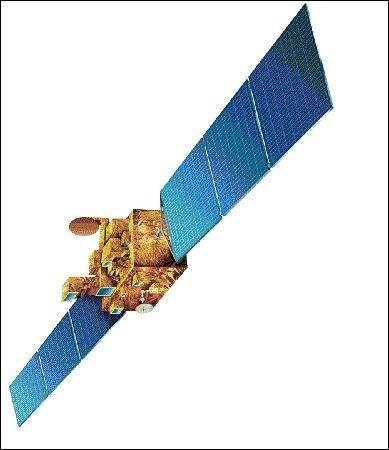
\includegraphics[scale=0.5]{image_gallery.png}
\caption{Ocean Sat}
\end{figure}
\chapter{Dynamic Model of spacecraft}
The dynamics for the spacecraft is modelled using Euler angles since the spacecraft is expected to operate within small ranges of Euler angles(Earth pointing satellite) and it is easier to design controller for euler angles.\\ \\
\textbf{Coordinate system} used(as given in the question):\\
Z axis-Pitch\\
Y axis-Roll\\
X axis-Yaw\\
Order of rotation is 3-2-1(z-y-x)\\
where,\\
yaw axis points towards Earth. Roll angle is in the direction of motion of the satellite and pitch axis as per right hand coordinate system.
\\ \\
The \textbf{Dynamics Equations} of motion for the spacecraft are given as follows.\\
\begin{equation}
I\dot{\omega}+\omega\times I(\omega)=T_{disturbance}+T_{magnetic}-T_{RW}+T_{g}
\end{equation}

\begin{equation}
\omega=\left(\omega_{b}-C_{b0}\begin{bmatrix}
0\\0\\\omega_{0}
\end{bmatrix}\right)
\end{equation}
Where,\\
	$ T_{magnetic} $ represents torque by magnetic torquers due to momentum dumping \\
	$ T_{RW} $ represents torque due to reaction wheels.\\
	$ T_{g} $ represents torque due to gravity gradient.\\
	$ \omega $ represents angular velocity of satellite wrt inertially fixed frame and written in body frame.\\
	$ \omega_b $ represents angular velocity of satellite wrt orbit and written/represented in body frame.

\section{Reaction wheel Torque:}
\subsection{Traditional Configuration:}
For reaction wheels in Traditional configuration, the net torque due to the wheels come out as,
\begin{equation}
T_{RW}=I_{w}\begin{bmatrix}
\dot{\omega_{1}}-\frac{\omega_{4}}{\sqrt{3}}\\
\dot{\omega_{2}}-\frac{\omega_{4}}{\sqrt{3}}\\
\dot{\omega_{3}}-\frac{\omega_{4}}{\sqrt{3}}
\end{bmatrix}
+I_{w}\begin{bmatrix}
\omega_{3}\omega_{by}-\omega_{2}\omega_{bz}\\
\omega_{1}\omega_{bz}-\omega_{3}\omega_{bx}\\
\omega_{2}\omega_{bx}-\omega_{1}\omega_{by}
\end{bmatrix}
\end{equation}
Where, \\
$\omega_{i}-$angular velocity of wheels wrt to the satellite. In normal operation all $\omega_{i}$ will be positive. Sign convention is taken so. \\
$ \omega_{b}- $(angular velocity of satellite body wrt orbit) is given by,\\
$
\omega_{b} =\begin{bmatrix}
-sin(r) & 0 & 1\\
cos(r) sin(y)&cos(y)&0\\
cos(r) cos(y)&-sin(y)&0
\end{bmatrix}
$ $
\begin{bmatrix}
\dot{p}\\ \dot{r} \\ \dot{y}
\end{bmatrix}
 $\\ \\
where [$\textbf{x}$,$\textbf{y}$,$\textbf{z}$]  correspond to the yaw(y), roll(r) and pitch(p) axes respectively and $ C_{b0} $ corresponds to the rotation matrix by,
\begin{equation}
C_{b0}=C_{x}(y)C_{y}(r)C_{z}(p)
\end{equation}
by the 3-2-1 rotation convention.
\newpage
\textbf{Note:} Second term of the reaction wheel torque will be small during operation(zero initially when rpms are 1000,1000,1000,1732). So it is only used in the simulink simulation and not in the controller design.
\subsection{Tetrahedron Configuration:}
\section{Gravity Gradient Torque:}
The gravity gradient torque is given by,
	\begin{equation}
	T_{g}=\frac{3\mu}{r^{5}}r_{b}^{\times}Ir_{b}=3\omega_{0}^{2}\begin{bmatrix}
	(I_{z}-I_{y})y\\(I_{z}-I_{x})r \\0
	\end{bmatrix}
	\end{equation}
	Where $ \omega_{0} =\sqrt{\frac{\mu}{R_{0}^{3}}}$.\\
This torque is only used in the final simulation of satellite with the controller and not used in the design of controller.
\section{Magnetic Torque}
The magnetic torque is based on a magnetic dipole system model of the earth where the satellite is in orbit about. Hence, for any point in the orbit, the magnetic field around the satellite can be easily found using the model and assuming that the dipole is aligned at angle of 11$ ^{0} $ wrt earth's true axis, we find the radial and azimuthal fields to be,
\begin{equation}
B_{r}=-2B_{0}\left(\frac{R_{E}}{r}\right)^{3}cos(\theta)
\end{equation}
\begin{equation}
B_{\theta}=-B_{0}\left(\frac{R_{E}}{r}\right)^{3}sin(\theta)
\end{equation}
\begin{equation}
|B|=B_{0}\left(\frac{R_{E}}{r}\right)^{3}\sqrt{1+3cos^{2}(\theta)}
\end{equation}
where, $ R_{E} $ is the mean radius of the earth, $ \theta $ is the azimuth from the north magnetic pole,r is the distance from earth's center and $B_{0}=3.12\times10^{-5}T$. There is no need to consider solar wind effects since the satellite OCEANSAT revolves closely about earth.
\chapter{Stability analysis}
Deriving the equations of motion, we get (The equations of motion remain same, but [$I_{x},I_{y},I_{z}$] of new frame become [$I_{y},I_{z},I_{x}$] of old frame.\\
Hence, the equations for stability come out to be,
\begin{equation}
I_{y}\ddot{r}-[I_{y}-I_{z}+I_{x}]\omega_{0}\dot{y}+4\omega_{0}^{2}(I_{z}-I_{x})r=0
\end{equation}
\begin{equation}
I_{z}\ddot{p}+3\omega_{0}^{2}(I_{y}-I_{x})p=0
\end{equation}
\begin{equation}
I_{x}\ddot{y}-[I_{y}-I_{z}+I_{x}]\omega_{0}\dot{r}+\omega_{0}^{2}(I_{z}-I_{x})r=0
\end{equation}

\section{Stability of pitch motion}
For stability of pitch, which has the form,
\begin{equation}
\ddot{p}+\alpha p=0
\end{equation}
$ \alpha>0 $ and hence $ I_{y}>I_{x} $. This is not true and hence the satellite is pitch unstable.
\section{Roll and yaw unstability}
In similar fashion, we see that if $ I_{z}>I_{x},I_{y} $, roll yaw is stable. However, by given info, the roll yaw is unstable. Hence, the satellite is gravity gradient unstable. 
\section{Need for active control}
The active control system is needed because of the unstable roll yaw motion and pitch motion. Because of constant disturbance torque given in the question. Dumping of Momentum gained will be required. This is done using 3 axis torque rods on satellite
\chapter{Controller design:}
\section{Linearised Dynamics Equations:}
\section{Controller Design:}
\begin{figure}[H]
\centering
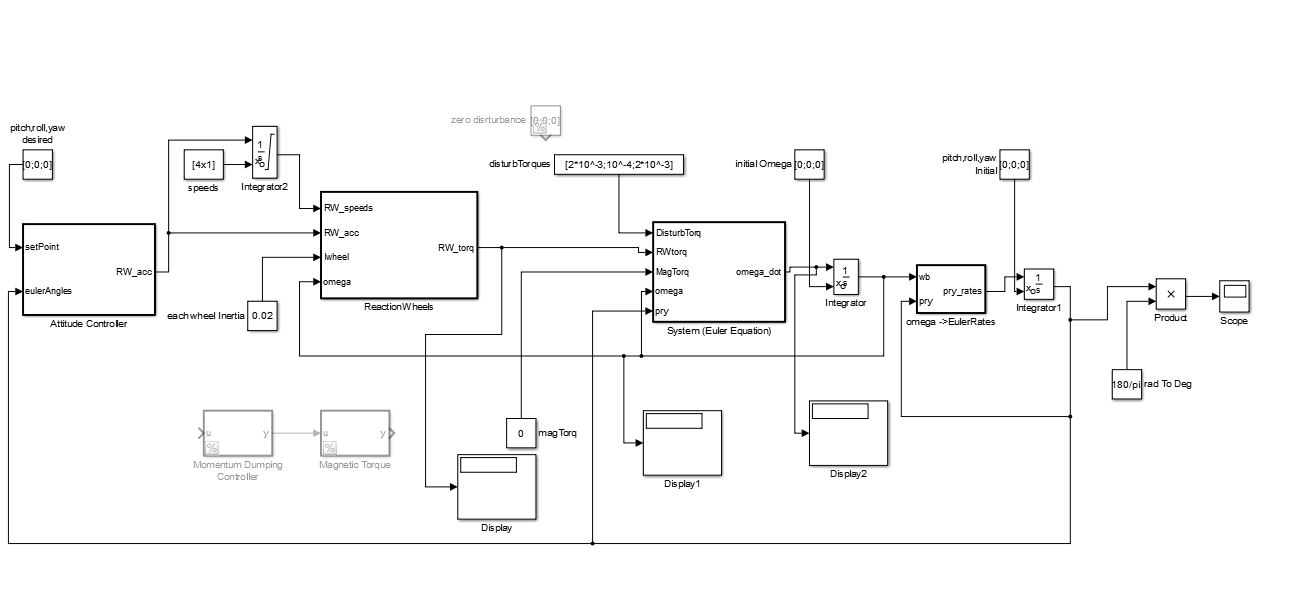
\includegraphics[scale=0.3]{Untitled1.png}
\caption{PID model}
\end{figure}

\chapter{Momentum Dumping:}
\end{document}